\section{}
% Make one plot showing the bridge output voltage (Δ𝐸0
% ) on the y-axis vs theoretical 
% strain on the x-axis. (Plot all the data including the repeated measurements at 1 kg.) 
% Fit each curve with a linear trendline with a zero intercept to find the sensitivity for 
% each bridge. Which bridge has the highest sensitivity? Why does it have the highest 
% sensitivity?


\subsection{Plot of Bridge Output Voltage vs Theoretical Strain}
The plot of bridge output voltage vs theoretical strain is shown in Figure \ref{fig:Q3Plot}.
\begin{figure}[h]
    \centering
    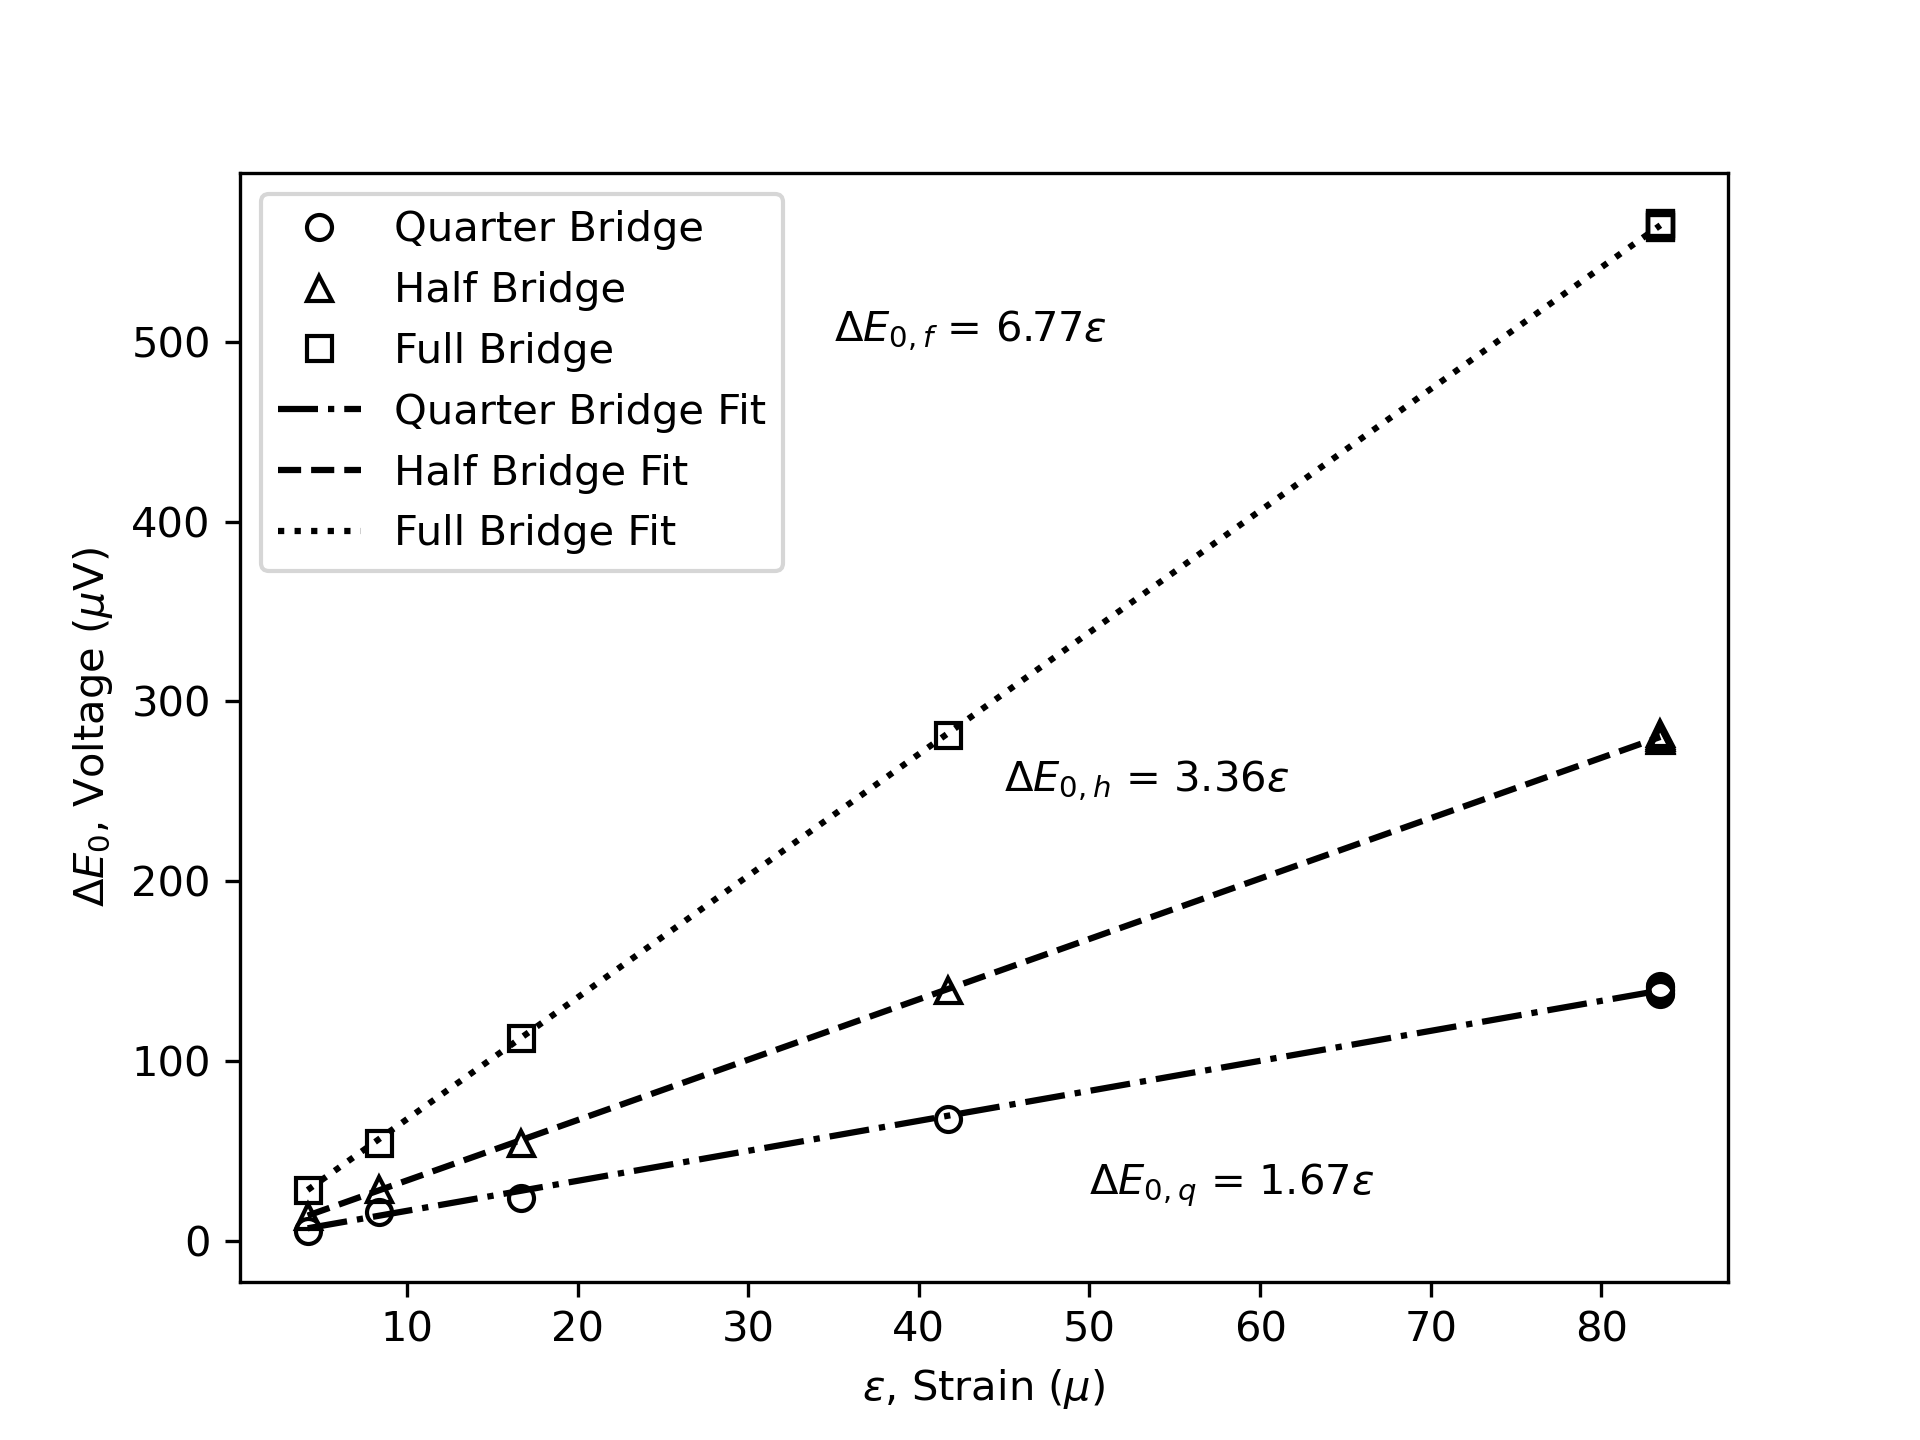
\includegraphics[width=0.8\linewidth]{matplotlib/Q3.png}
    \caption{Plot of bridge output voltage vs theoretical strain}
    \label{fig:Q3Plot}
\end{figure}

\subsection{Sensitivity of Each Bridge}
The sensitivity of each bridge is given in Table \ref{tab:Q3Sensitivity}.

\begin{table}[h]
    \centering
    \caption{Sensitivity of each bridge}
    \label{tab:Q3Sensitivity}
    \begin{tabular}{cc}
        \toprule
        Bridge & Sensitivity \\
        & (V) \\
        \midrule
        Quarter Bridge & 1.67 \\
        Half Bridge & 3.36 \\
        Full Bridge & 6.77 \\
        \bottomrule
    \end{tabular}
\end{table}
\FloatBarrier
\subsection{Discussion}
The full bridge has the highest sensitivity because it has the most strain gauges. For example,
a displacement on the top will increase the measurement of the strain gauges $\epsilon_1$ and $\epsilon_4$. 
A displacement on the bottom will increase the measurement of the strain gauges $\epsilon_2$ and $\epsilon_3$.
This results in $\epsilon_1 - \epsilon_2 - \epsilon_3 + \epsilon_4 = 4 \epsilon$.

The least sensitive bridge is the quarter bridge because it only has one strain gauge. A displacement on the top
will increase the measurement of the strain gauge $\epsilon_1$. None of the other strain gauges will be affected.
This results in $\epsilon_1 = \epsilon$.z